\section{How it's different from Word}
    \subsection{WYSIWYG - What You See Is What You Get}
        You may be familiar with the challenge that is using Word to write equations even as simple as those in Figure \ref{fig:word}.

        \begin{figure}[h]
            \centering
            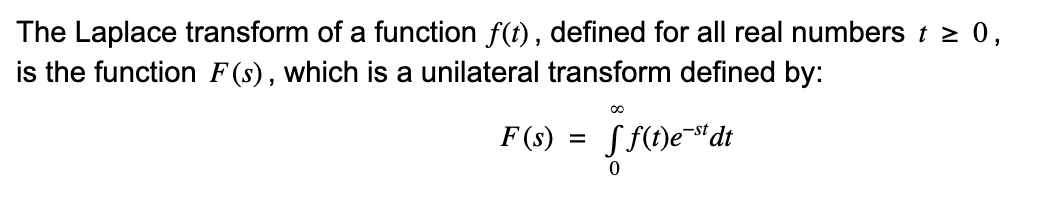
\includegraphics[scale=0.8]{figures/word.png}
            \caption{Word, an example of What You See Is What You Get}
            \label{fig:word}
        \end{figure}

        The text, in the exact way it's seen, is all the information we have.
        This is often called ``What You See Is What You Get'', or WYSIWYG for short, and refers to popular word processing programs like Word, Pages, and so on.
        While there is a place for them, think of it as focused on only producing text, and everything else is secondary.

        In writing scientific papers, well typeset equations, diagrams, etc are a must.
        For this, we can use more specialised software that handles everything exactly using code, instead of visually approximating.

    \subsection{Typesetting}
        \LaTeX, pronounced either \emph{lah-tec} or \emph{lay-tec}, is a collection of separate programmes which take plain text and instructions and output beautifully typeset documents.
        One of these programmes is \TeX, and it handles most of the actual typesetting (e.g. exact spacing between equatins, etc), allowing us to focus on content.

        The main motivators for why you would want to use it are:
        \begin{enumerate}
            \item Beautifully written documents. No more trying to deal with the various fonts, margins, spacing, etc.
            \item Easy bibliography management, citations and cross-references
            \item Easily typed equations and graphs. Even complicated maths can be easily organised and written.
        \end{enumerate}

        Let's go back to our example, and see how it would be done with \LaTeX:
        \lstinputlisting[language=TeX, label=ls:Laplace, caption=Example document written with \LaTeX]{files/introduction/example1.tex}
        Resulting in:\\
        The Laplace transform of a function $f(t)$, defined for all real numbers $t \geq 0$ is the function $F(s)$, which is a unilateral transform defined by:
        \begin{equation*}
            F(s) = \int_0^\infty f(t)e^{-st} dt
        \end{equation*}

        If you are familiar with programming, this may remind you of a \emph{markup} language, and that's exactly what it is!
        In short, we have a plain text file saved in \texttt{.tex} that contains instructions on how to compile it to \texttt{.pdf}.
        Inbetween that we see the actual content for the document.

        Let's briefly explore some key \LaTeX\ concepts.
        Don't worry about fully understanding them now.
        At this stage, the purpose is simply understanding what to expect.

\section{Markup language}
    Plain text is written like plain text, but most of LaTeX's power comes from its markups.
    A backslash, \verb|\|, creates a markup; curly brackets \verb|{}| indicate an \emph{argument}, and square brackets \verb|[]| (optionally) provide options.
    So \verb|\section{Introduction}| would create an Introduction header. 

    Generally, we are either creating an environment, defining instructions or using variables:

    \paragraph{Environments}
    introduce some kind of formatting, such as lists, math mode or more complicated things.
    With very few exceptions, environments have the following format:
        
    \begin{lstlisting}
\begin{environment-name}[options]
    ...
\end{environment-name}
    \end{lstlisting}
        
    In our example, we created both the required \texttt{document} environment, and the math display \texttt{equation*}.
        
    \paragraph{Instructions}
    define some feature of the document. This ranges from breaking a page, to creating double-spacing, defining the document's class, and much more. In our example you can see:

    \verb|\documentclass[...]{article}|
        
    \paragraph{Variables}
    range from greek letters to the integral sign to a whole expression.
    Some examples seen are \verb|\geq| (\textbf{g}reater or \textbf{eq}ual) and \verb|\int| ($\int$).
    Intuitively, \verb|\alpha| results in $\alpha$, and they can even be user-defined.
        
    \paragraph{Note:}
    Like other programming languages, there are certain reserved characters with predefined meaning, such as \verb|\|, \verb|{|, \verb|}| and \verb|&|.
    To use the literal curly brackets, ampersand, etc we would need to \emph{escape} them.
    Conveniently, this is done with a backslash (\verb|\|), so feel free to think of them as variables: \verb|\{|, \verb|\}| and \verb|\&|.

\section{Packages}
    You may have noticed that \verb|\usepackage{amsmath}| was not mentioned as an instruction the previous section. That's because packages are worth mentioning on their own.

    Packages add features to our document, similar to \emph{import} in most programming languages.
    \verb|amsmath| gives us a wide array of maths tools, but there are packages for drawing, graphing, colouring, better management of bibliography, easier organisation of your files, and so on.
    
\section{Compilation}
    As mentioned previously, \LaTeX\ documents are written in plain text with a set of instructions.
    This means that our \texttt{.tex} files can be written in any text editing software \verb|.tex|, and to produce the output \verb|.pdf|, it needs to be \emph{compiled}.

    You may spend a lot of time scratching your head, wondering what is wrong with your code and why it's not compiling.
    We very specifically will avoid most of the programming side of \TeX, which is some kind of macro expansion language.
    You will still run into some challenges, but they tend to be forgetting a bracket, rather than unexpected behaviour.

    We are not going to focus on the various compilers, and just use \texttt{latexmk}, or whichever is default in your distribution.
    The good news is that the recommended IDEs (\textbf{I}ntegrated \textbf{D}evelopment \textbf{E}nvironments, basically text editors filled with features) handle the compilation for you and have features to help you spot mistakes.